%-----------------------------------------------------------------------------%
% Document class
%-----------------------------------------------------------------------------%
\documentclass[a4paper,12pt,onecolumn,final]{article}
%-----------------------------------------------------------------------------%
% Geometry package for setting page margins
%-----------------------------------------------------------------------------%
\usepackage[paper=a4paper,vscale=0.8,hscale=0.85,centering]{geometry}
%-----------------------------------------------------------------------------%
% Helvet package for font
%-----------------------------------------------------------------------------%
\usepackage[scaled=0.92]{helvet}
\renewcommand{\familydefault}{\sfdefault}
%-----------------------------------------------------------------------------%
% Include special packages here
%-----------------------------------------------------------------------------%
\usepackage{amsmath,amsfonts,amssymb}
\usepackage{xcolor}
\usepackage{graphicx}
\usepackage{hyperref}
\usepackage{listings}
\lstset {backgroundcolor=\color{black!5}, basicstyle=\footnotesize, stringstyle=\color{red}, commentstyle=\color{green!50!black}, basicstyle=\footnotesize\ttfamily, keywordstyle=\color{blue}, 
}
%-----------------------------------------------------------------------------%


%-----------------------------------------------------------------------------%
\begin{document}
%-----------------------------------------------------------------------------%


%-----------------------------------------------------------------------------%
\noindent
\begin{tabular}{|p{0.2\textwidth}|p{0.75\textwidth}|}
\hline
\textbf{G14CAM} & \textbf{Computational Applied Mathematics}
\\
2017--2018 & \textcolor{red}{Coursework 1 Part B}
\\
\hline
\textbf{Name} & \textcolor{red}{Ella Taylor}
\\ 
\textbf{Student ID} & \textcolor{red}{4290562}
\\ 
\textbf{Date} & \today
\\
\hline
\textbf{Existing codes} & \textcolor{red}{Names of approved existing codes that you used}
\\
\hline
\end{tabular}
%-----------------------------------------------------------------------------%
% \textcolor{red}{LaTeX instruction: This TeX-file template can be compiled using PDFLaTeX.}
%-----------------------------------------------------------------------------%
\section*{Problem 1}

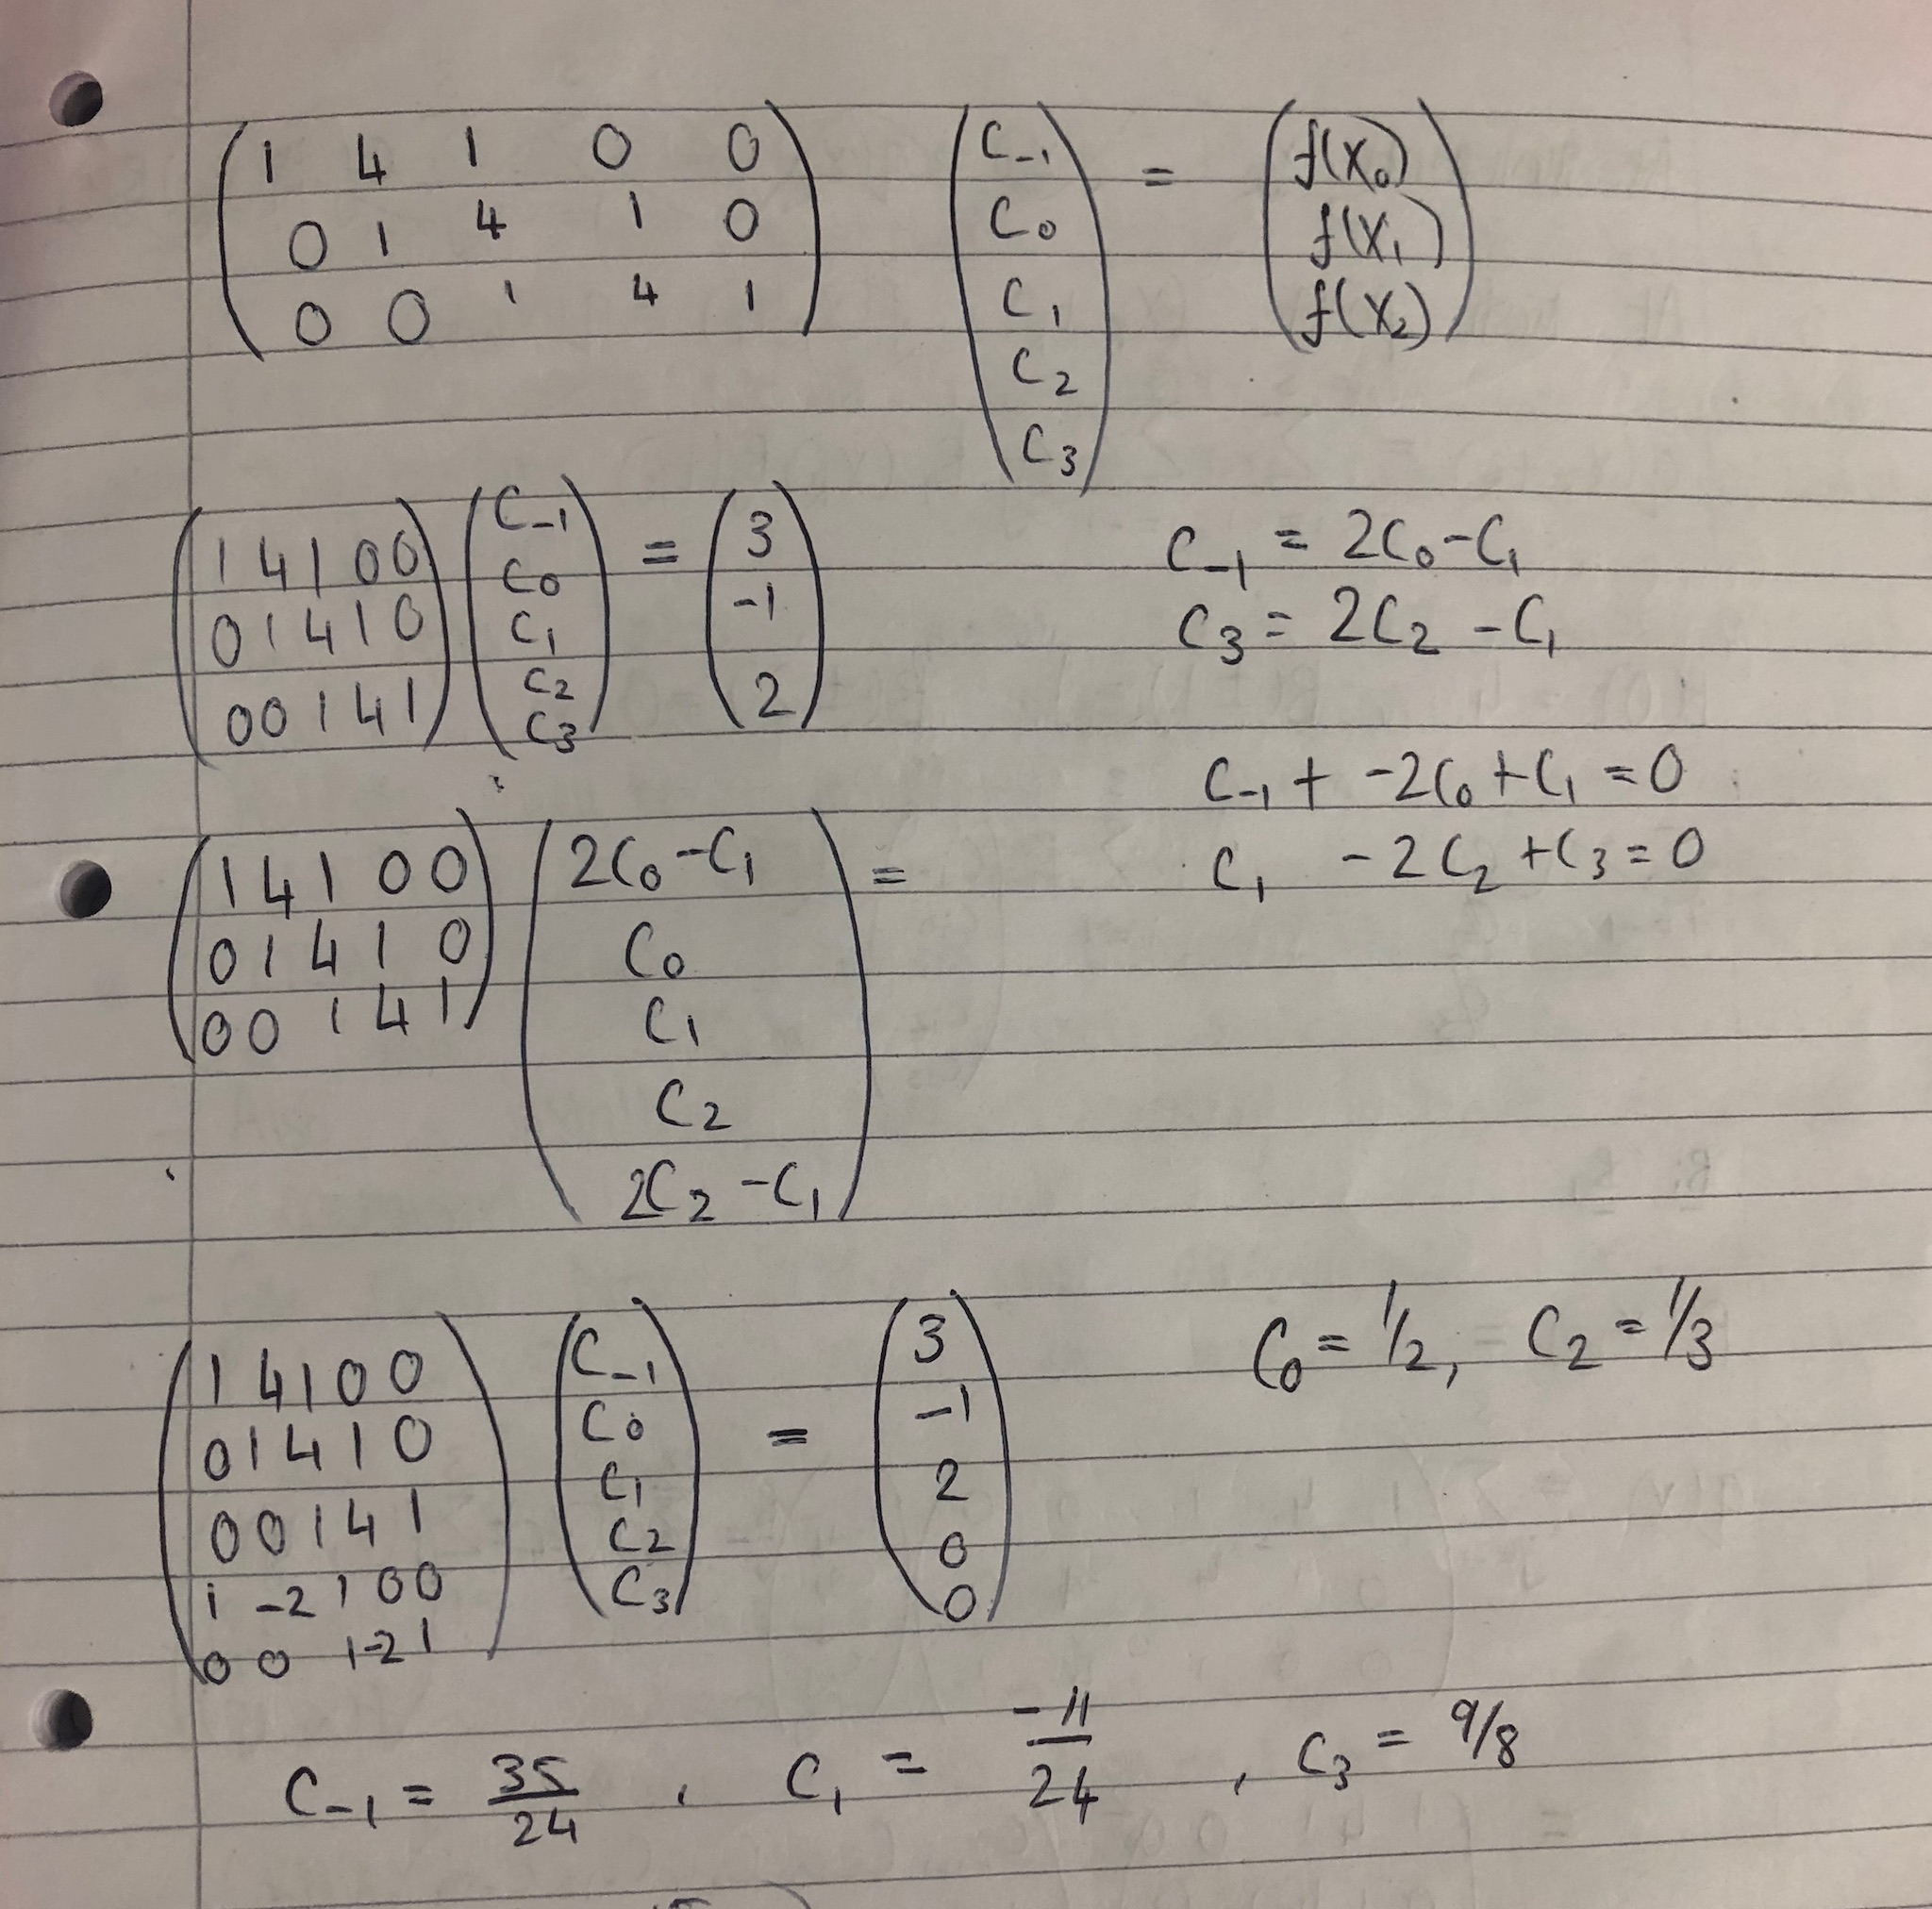
\includegraphics[scale=0.25]{cw1bQ1.jpg} 

%-----------------------------------------------------------------------------%
\section*{Problem 2}
\subsection*{Problem 2.A}

\begin{lstlisting}[language=C++]
#include <iostream>
#include <cmath>
#include <iomanip>

void tridiagonal_matrix_solver(int n, double* c, double* lower, double* diag, 
double* upper, double* f);

int main()
{
double h; //stepsize
std::cout<<"Enter stepsize h \n";
std::cin>>h;
double L; //Length of  interval
std::cout<<"Enter length of interval (0,L) \n";
std::cin>>L;
int n; //n is the number of nodes
n = int((L/h) +1.0);

double x[n];
double pi = 3.14159265358979323846;

double* lower;
lower = new double[n-1];

double* diag;
diag = new double[n];

double* upper;
upper = new double[n-1];

double* f;
f = new double[n];

for (int i=0; i<n; i++)
    {
    x[i] = 0.0 + h*(double)(i); //Interval (0,l)
    f[i] = exp(x[i])*sin((5.0/4.0)*pi*x[i]); //f(x) = exp(x)*sin(5pi/4)x)
    }


f[0]   = f[0] + (h/3.0)*exp(x[0])*(sin(5.0*pi*x[0]/4.0)+
(5.0*pi/4.0)*cos(5.0*pi*x[0]/4.0));
f[n-1] = f[n-1] - (h/3.0)*exp(x[n-1])*(sin(5.0*pi*x[n-1]/4.0)+
(5.0*pi/4.0)*cos(5.0*pi*x[n-1]/4.0));

//f dash evaluated at end points
double f_diff[2];
f_diff[0] = exp(x[0])*(sin(5.0*pi*x[0]/4.0)+(5.0*pi/4.0)*cos(5.0*pi*x[0]/4.0));
f_diff[1] = exp(x[n-1])*(sin(5.0*pi*x[n-1]/4.0)+
(5.0*pi/4.0)*cos(5.0*pi*x[n-1]/4.0));

double* c;
c = new double[n]; //c not including c[-1] and c[n+1]

c[0] = 0.0;
diag[0] = 4.0;
upper[0] = 2.0;
lower[n-2] = 2.0;
diag[n-1] = 4.0;
c[n-1] = 0.0;

for (int i=1; i<n-1; i++)
    {
    c[i] = 0.0;
    lower[i-1] = 1.0;
    diag[i] = 4.0;
    upper[i] = 1.0;
    }

tridiagonal_matrix_solver(n,c,lower,diag,upper,f);

//Printing out entries of c
double c_end[n+2]; //c including end values

c_end[0] = c[2] - (1.0/3.0)*h*f_diff[0];
c_end[n+1] = c[n-2]+(1.0/3.0)*h*f_diff[1];

std::cout<<"c[-1] = "<<c[0]<<"\n";
for( int i = 0; i<n; i++)
{
c_end[i+1] = c[i];
std::cout<<"c["<<i<<"] = "<<c_end[i+1]<<"\n";
}
std::cout<<"c["<<n<<"] = "<<c_end[n+1]<<"\n";

delete[] lower;
delete[] upper;
delete[] diag;
delete[] f;
delete[] c;

return 0;
}
\end{lstlisting}%


%-----------------------------------------------------------------------------%
\subsection*{Problem 2.B}
\begin{center}
\begin{tabular}{cr}
\hline\hline
 $i$ & $c_i$
\\
\hline
-1 & -0.132442
\\
0 & -0.0155912
\\
1 & 0.194807
\\
2 & 0.303991
\\
3 & 0.112447
\\
4 & -0.340775
\\
5 & -0.671465
\\
6 & -0.396644
\\
7 & 0.542973
\\
8 & 1.42184
\\
9 & 1.15873
\\
\hline\hline
\end{tabular}
\end{center}
%-----------------------------------------------------------------------------%
\subsection*{Problem 2.C}
\begin{center}
\begin{tabular}{c|cc}
 $h$ & $q_h(\frac{1}{3})$ & $\big|f(\frac{1}{3}) - q_h(\frac{1}{3})\big|$
\\[0.5ex]
\hline
$1/2$ & $0.654498$	& $0.69356$ 
\\
$1/4$ & $1.06763$	& $0.28043$
\\
$1/8$ & $1.06763$	& $0.28043$
\\
$1/16$ & $1.28694$	& $0.0611199$
\\
$1/32$ &  $1.28694$	& $0.0611199$
\\
$1/64$ & $1.28694$	& $0.0611199$
\\
$1/128$ & $1.33343$	& $0.0146324$

\\
\end{tabular}
\end{center}


\begin{lstlisting}[language=C++]
#include <iomanip>
#include <iostream>
#include <cmath>
#include <cassert>

double evaluate_qh(int n, double h, double x_val, double x0, double* c)
{
double qh = 0;

//For any x in [xk-1,xk] bi is only locally non zero
//therefore q(x) = ck-2Bk-2(x) + ck-1Bk-1(x) + ckBk(x) + ck+1Bk+1(x)
int k = int((x_val - x0)/h +1.0);

assert(k>=0);

if (k<2)
    {
    qh = 4.0*c[k]+ 2.0*c[k+1];
    }
else if ((k>1) && (k<=n))
    {
    qh = c[k-1] +4.0*c[k]+c[k+1];
    }
else
    {
    qh = 2.0*c[k-1]+4.0*c[k];
    }
return qh;
}


void tridiagonal_matrix_solver(int n, double* x, double* lower, double* diag,
 double* upper, double* f);
double evaluate_qh(int n, double h, double x_val, double x0, double* c);

int main()
{
double h; //stepsize
double L = 2; //Length of  interval
int n; //n is the number of nodes
double pi = 3.14159265358979323846;

double x_val;
std::cout<<"Enter x \n";
std::cin>>x_val;
double q_h;
double Err = 0;

std::cout << "-------------------------------------------
-------------------------------"
            << std::endl;

std::cout << std::setw(10) << "h"
              << std::setw(20) << "q_h"
              <<std::setw(40) << "Err"
              << std::endl
              << "-------------------------------------------
            -------------------------------"
            << std::endl;
double* x;
double* lower;
double* diag;
double* upper;
double* f;
double* c;
double* c_end;

double f_diff[2];
f_diff[0] = exp(x[0])*(sin(5.0*pi*x[0]/4.0)+(5.0*pi/4.0)*cos(5.0*pi*x[0]/4.0));

for (int j = 1; j<15; j++)
    {

    h = pow(0.5,j);
    n = int((L/h) +1.0);
    x = new double[n];
    lower = new double[n-1];
    diag = new double[n];
    upper = new double[n-1];
    f = new double[n];
    c = new double[n];
    c_end = new double[n+2]; //c including end values

    for (int i=0; i<n; i++)
        {
        x[i] = 0.0 + h*(double)(i); //Interval (0,l)
        f[i] = exp(x[i])*sin((5.0/4.0)*pi*x[i]); //f(x) = exp(x)*sin(5pi/4)x)
        }
    f[0]   = f[0] + (h/3.0)*exp(x[0])*(sin(5.0*pi*x[0]/4.0)+
    (5.0*pi/4.0)*cos(5.0*pi*x[0]/4.0));
    f[n-1] = f[n-1] - (h/3.0)*exp(x[n-1])*(sin(5.0*pi*x[n-1]/4.0)+
    (5.0*pi/4.0)*cos(5.0*pi*x[n-1]/4.0));

    c[0] = 0.0;
    diag[0] = 4.0;
    upper[0] = 2.0;
    lower[n-2] = 2.0;
    diag[n-1] = 4.0;
    c[n-1] = 0.0;

    for (int i=1; i<n-1; i++)
        {
        c[i] = 0.0;
        lower[i-1] = 1.0;
        diag[i] = 4.0;
        upper[i] = 1.0;
        }

    tridiagonal_matrix_solver(n,c,lower,diag,upper,f);

    f_diff[1] = exp(x[n-1])*(sin(5.0*pi*x[n-1]/4.0)+
    (5.0*pi/4.0)*cos(5.0*pi*x[n-1]/4.0));

    c_end[0] = c[2] - (1.0/3.0)*h*f_diff[0];
    c_end[n+1] = c[n-2]+(1.0/3.0)*h*f_diff[1];


    for( int i = 0; i<n; i++)
    {
    c_end[i+1] = c[i];
    }

    q_h = evaluate_qh(n,h,x_val,x[0],c_end);

    Err = fabs(exp(1.0/3.0)*sin(pi*5.0/12.0) - q_h);


    std::cout<< std::setw(10)<<h
    <<std::setw(20)<<q_h
    <<std::setw(40)<<Err<<std::endl;

    }

delete[] lower;
delete[] upper;
delete[] diag;
delete[] f;
delete[] c;
delete[] x;
delete[] c_end;
}


\end{lstlisting}%

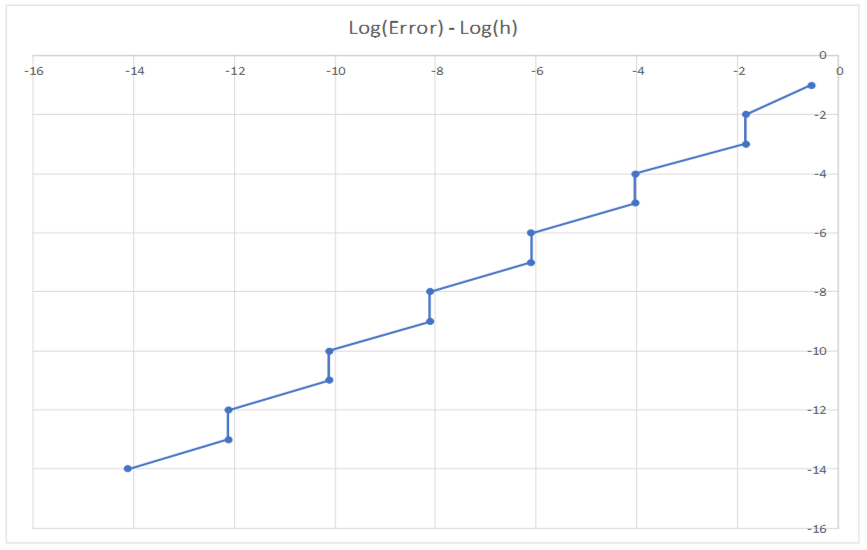
\includegraphics[scale=1]{CW1bGRAPH.png} 

\begin{verbatim}
Gradient is roughly one, so step size is related to convergence by order one.
\end{verbatim}

%-----------------------------------------------------------------------------%
\section*{Problem 3}

\\
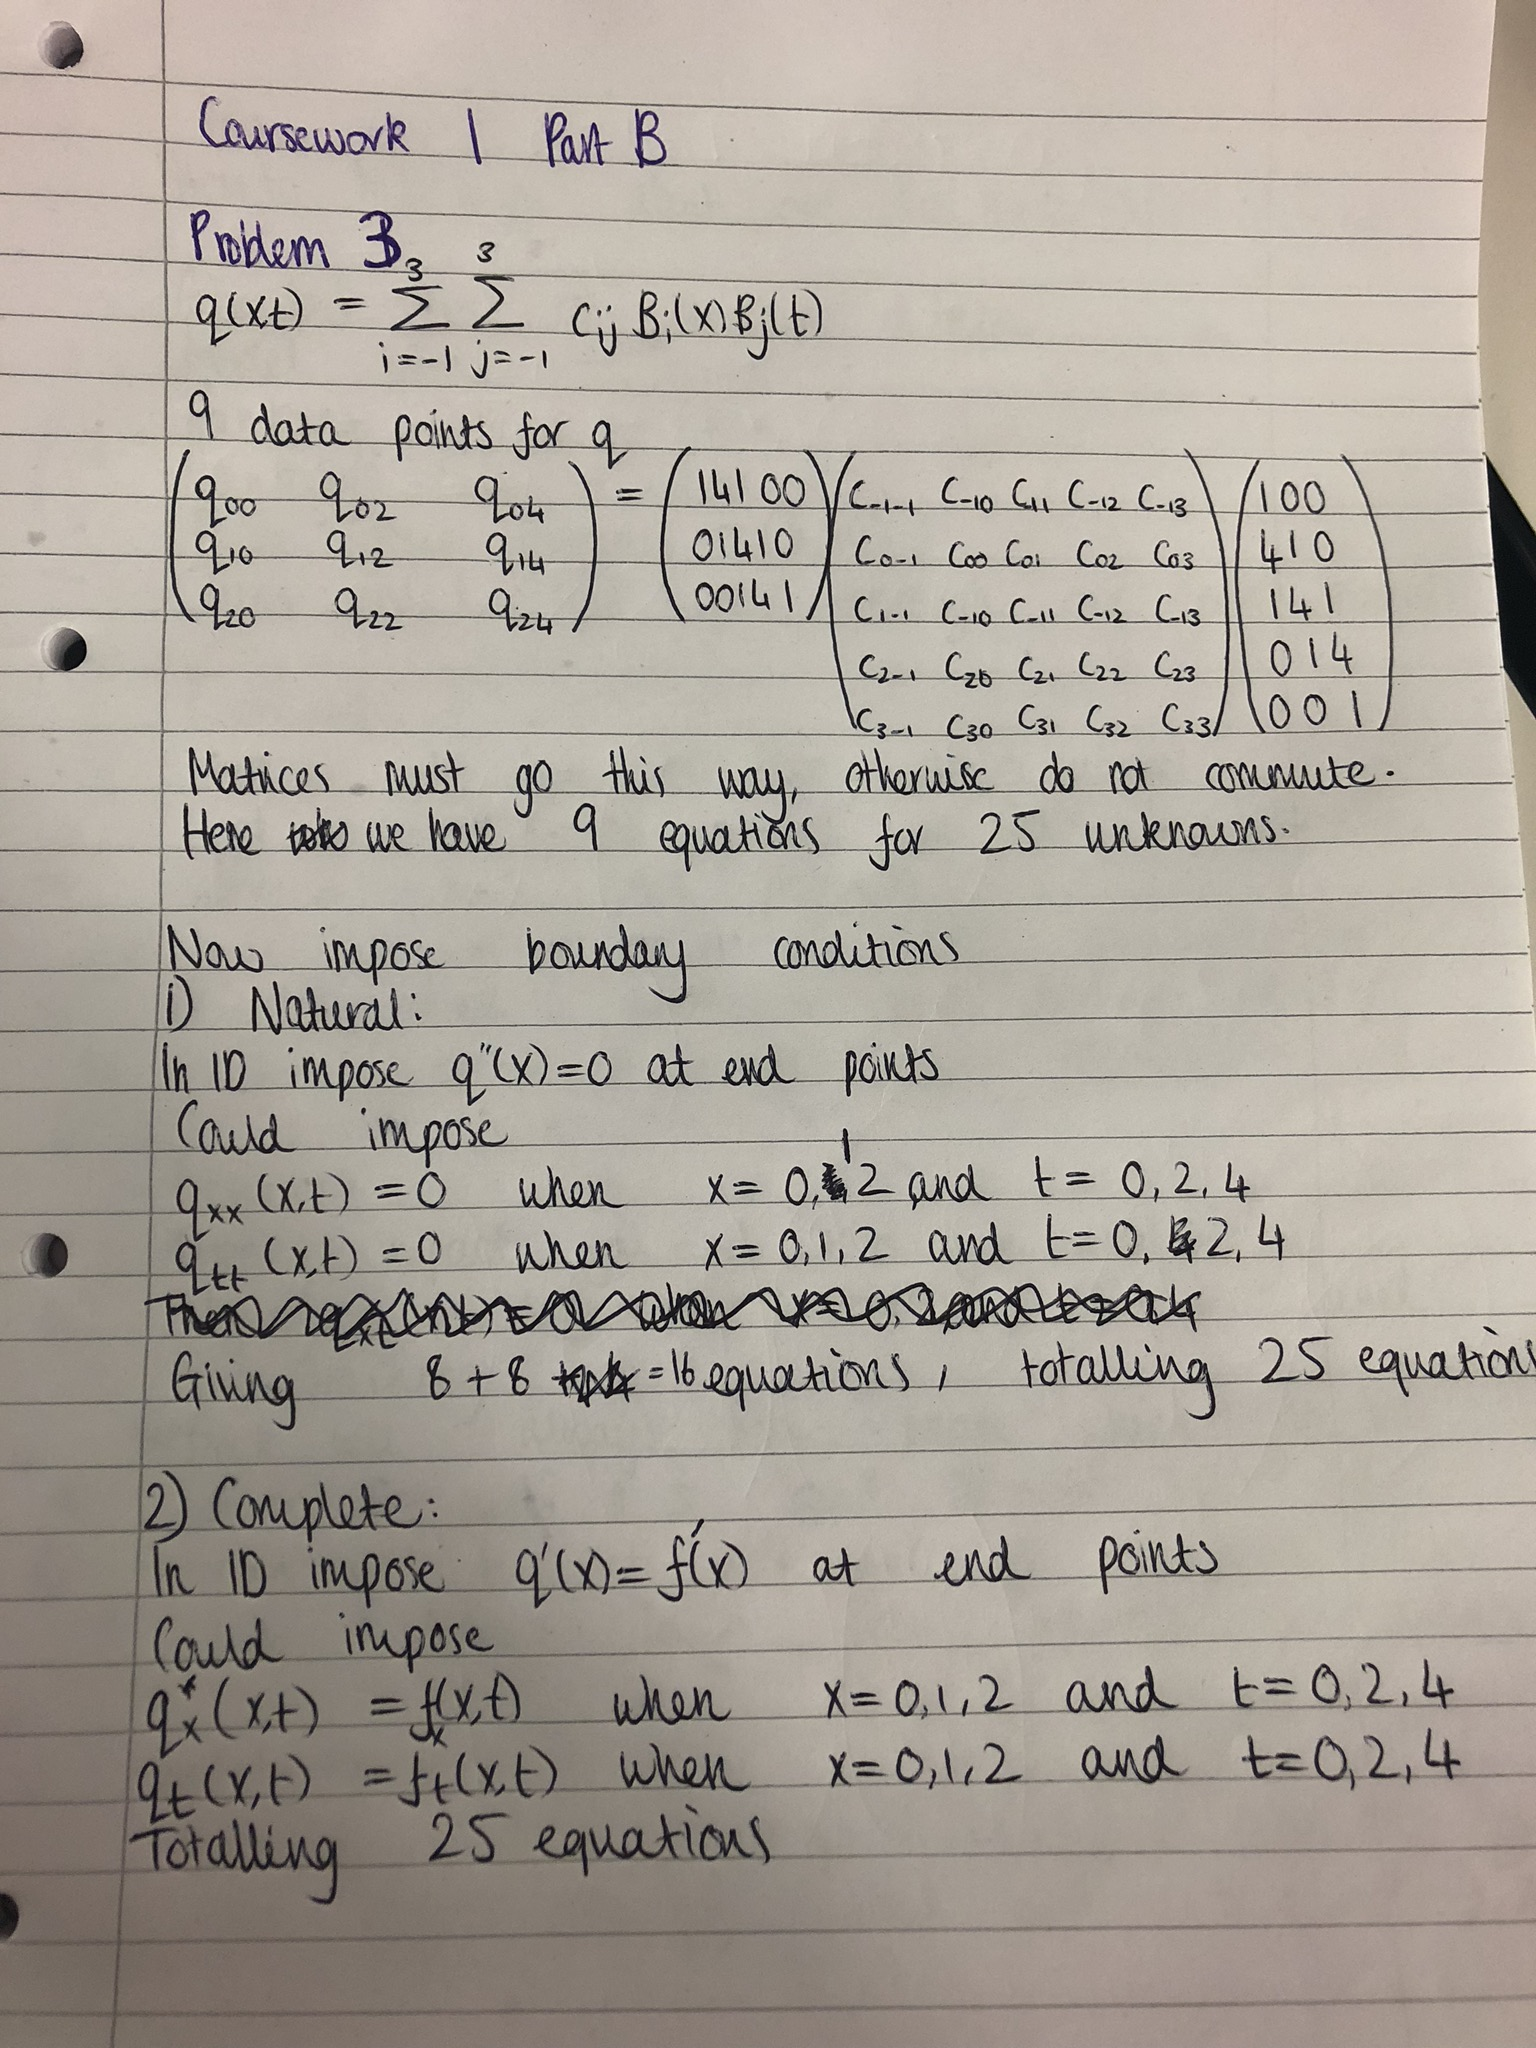
\includegraphics[scale=0.3]{cw1bQ3.jpg} 

%-----------------------------------------------------------------------------%
\end{document}
%-----------------------------------------------------------------------------%
